\section{Introduction}
Memory Networks (MemNN) \citep{weston2014memory} are a class of learning models
that combine inference with long-term memory. Unlike Recurrent Neural Networks
(RNN) that model language \citep{mikolov2010recurrent}, and their variants with
Long Short-Term Memory (LSTM) \citep{hochreiter1997long}, MemNNs store a global
memory with read and write functions. While MemNN required explicit supervision
for selecting the relevant parts of the memory, \citep{sukhbaatar2015end}
proposed a end-to-end variant (MemN2N) where the memory selection component is
trained jointly with the rest of the network. These were previously used for
answering questions that require reasoning over multiple background sentences,
both in simulated \citep{bordes2010towards} and large-scale
\citep{fader2013paraphrase} scenarios. In this work, we apply MemN2N to the task
of answering science questions. This dataset is significantly different from the
QA datasets previously used to test memory networks, and requires more complex
reasoning. One example of such question is shown below.
%TODO(pradeep): Make this a table?
\begin{itemize}
\item \textit{Astronauts weigh more on Earth than they do on the moon because \\
(A) they have less mass on the moon (B) their density decreases on the moon (C)
the moon has less gravity than Earth (D) the moon has less friction than Earth}
\end{itemize}
%TODO(pradeep): Say more things about the nature of the problem.
In this chapter, we take a generic view of MemN2N as shown in
Figure~\ref{fig:memnet} and identify five configurable components in it:
\textit{query encoder}, \textit{background encoder}, \textit{memory selector},
\textit{memory updater} and an \textit{answer prediction} module, all
implementing appropriate functions. We experiment with various configurations of
these components and show results on the science QA dataset. It has to be noted
that given good representations of the question, candidate answers and
background information, QA can be seen as a textual entailment problem.
Following this observation, we pretrain the encoders and the entailment module
using Stanford's Natural Language Inference (SNLI) dataset
\citep{bowman2015large}.

\section{Approach}
\begin{figure*}
\begin{center}
  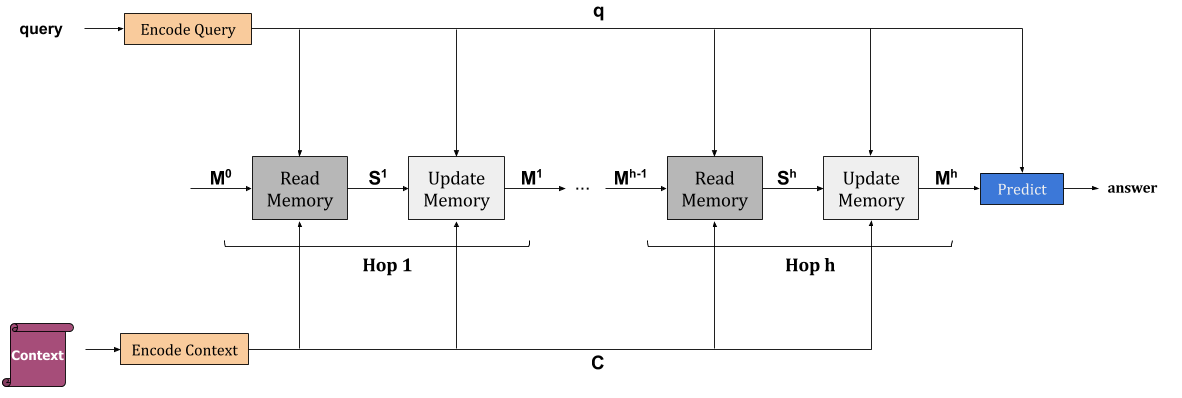
\includegraphics[width=6in]{figures/memory_network_generic.png}
  \caption{Schematic showing a generic view of end-to-end memory network. The
gray boxes are the configurable components in our model.}
  \label{fig:memnet}
  \end{center}
\end{figure*}
\subsection{Memory Network Setup}
Figure~\ref{fig:memnet} shows the setup of our memory network model, which is a
generalization of the MemN2N model \citep{sukhbaatar2015end}. Our model takes as
input a set of $N$ background sentences indexed as $\{b_i\}_{i=1}^N$, such that
$b_i$ is a vector containing the indices of words in the $i^\text{th}$ sentence.
The sentences are then encoded using the \texttt{EncodeBackground} function to
produce the matrix $B \in \mathbb{R}^{n \times d}$, where each row $B[i]$ is the
encoding of sentence $b_i$. In addition, the model also takes as input a query
indexed as $q$, which is a vector containing the indices of the words in the
query similar to $b_i$ vectors. The query is encoded using \texttt{EncodeQuery}
to produce $u^0 \in \mathbb{R}^d$. The memory network can have multiple memory
layers, corresponding to multiple hops. At each hop, a memory layer receives as
input the output from the previous hop $u^{h-1}$, which is passed to the
\texttt{SelectMemory} function, which uses an attention mechanism to select the
relevant parts of the encoded background, conditioned on $u^{h-1}$ and produces
a summary $s^h$, of the background encoding for the current hop. $s^h$ is then
passed to \texttt{UpdateMemory} along with $u^{h-1}$, to produce the updated
memory representation $u^h$ for the current hop. It has to be noted that the
initial $u^0$ is the encoding of the query itself. Finally, an answer is
predicted by passing the query encoding $u^0$, and the summary of the
background, $s^H$ from the final hop $H$ to the \texttt{PredictAnswer} function.

It can be seen that MemN2N fits into this setup with the following
configuration:
% TODO(pradeep): MemN2N actually has two Embedding matrices encoding background
for input and output. Also, there is another variant which encodes positions of
the words too.
\begin{flalign*}
&\texttt{EncodeQuery}(q) = \text{Embedding}_q(q) \\
&\texttt{EncodeBackground}(b_i) = \text{Embedding}_b(b_i) \\
&\texttt{SelectMemory}(u^{h-1}, B) = \text{softmax}(B.u^{h-1}).B \\
&\texttt{UpdateMemory}(u^{h-1}, s^h) = u^{h-1} + s^h \\
&\texttt{PredictAnswer}(s^H) = \text{softmax}(W.s^H)
\end{flalign*}
where $\text{Embedding}_q(.)$ and $\text{Embedding}_b(.)$ are simply bag of
words models that aggregate the vector representations of all the words given by
the indices in the input. $W \in \mathbb{R}^{V \times d}$ is a parameter of the
answer prediction function, causing the softmax to be over the vocabulary size
$V$. Note that in MemN2N, $u^0$ is not an argument of \texttt{PredictAnswer}.

\paragraph{Science Question Answering as Textual Entailment} In our setup, we
transform the problem of answering science questions into a textual entailment
problem. That is, given a multiple choice question with answer options, we
convert the combination of the question and each of the options into a
statement, and check whether the statement can be entailed from relevant
background information. The datasets used are described in
Section~\ref{sec:data}. Given this setup, the \texttt{PredictAnswer} function
essentially becomes an entailment function.

\section{Preliminary Results}

\subsection{Analysis}

\section{Proposed Work}